\fancychapter{User studies}
\label{chapter:results}

In order to evaluate the created social robot on the game playing scenario of \emph{Sueca}, a user study was conducted.
The main idea was to set up the environment in which this robot is supposed to interact with human players, and collect, in an adequate way, their feelings and perceptions.
The targeting measures are the trust on the partner, the affect felt, and also the perception of the team player's social presence.
Therefore, participants answered a questionnaire before playing with \ac{emys} and another one after the game.
The current chapter starts with the samples description and proceeds with analyses on three mentioned measures.

\section{Samples Description}
\label{sec:samples}
A group of 60 participants were included in this study with a mean age of 24,31 $\pm$ 3,852.
Out of the 60 subjects, 40 played the game with a human partner and 20 played with \ac{emys} as their team player.
These distributions aimed to collect a valid number of answers from \ac{emys} partners.
Additionally, out of the 59 subjects that revealed their gender, 20 were females and 39 were males.
Furthermore, most participants affirmed to know their partners in spite of not having played with them before, and their \emph{Sueca} knowledge was nearly medium.

\section{Trust}
\label{sec:trust}
The trust in the partner was measured for each individual before and after the game session, with the Human-Robot Trust Questionnaire \cite{}.
Consequently, the following three questions arose:
\begin{itemize}
\item Are there changes in trust after the experience of interacting with the \emph{Sueca} partner?
\item Are the trust levels influenced by the partner (robot or human)?
\item Are the trust levels influenced by the game results?
\end{itemize}

\subsection*{Are there changes in trust after the experience of interacting with the \emph{Sueca} partner?}

The statistical test used to infer a conclusion about this question was a Mixed ANOVA, with time as a factor of 2 levels and condition (team player type) as the between-subjects factor.
Additionally, assumptions were tested to guarantee the data validity.
The dependent variable (time) showed a significant effect with p = 0.03.
However, by adding the independent variable (condition), the effect was not significant with p = 0.65.

\begin{figure}[h!]
  \centering
    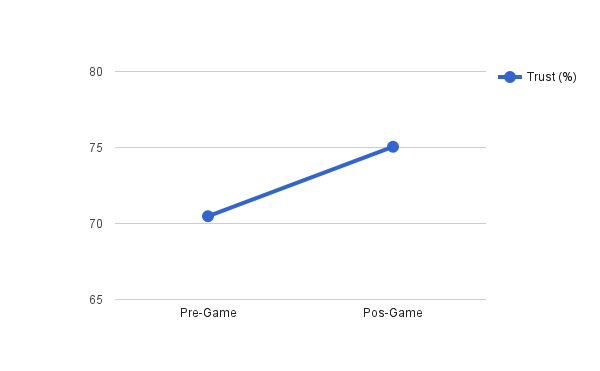
\includegraphics[width=0.7\textwidth]{./img/6/trustMixedANOVA}
  \caption{Evolution of the trust percentage between the two time levels}
\label{fig:trustMixedANOVA}
\end{figure}

Figure~\ref{fig:trustMixedANOVA} presents the evolution of the trust percentage between the two time levels, before the game and after the game.
The trust values correspond to estimated means separated by time, since it was the only significant variable.

\textbf{Answer:} There were significant differences in Trust before and after playing \emph{Sueca}, but there was not significant differences between \emph{Sueca} partners at different time levels.



\subsection*{Are the trust levels influenced by the partner (robot or human)?}

The statistical test used to infer a conclusion about this question was the Welch Test, with condition as factor and pos-game trust as dependent variable.
As a result, the condition effect was proved with p = 0, suggesting the means of trust were significantly different between having a robot partner or a human partner.

\textbf{Answer:} There were significant differences in Trust between different \emph{Sueca} partners.


\subsection*{Are the trust levels influenced by the game results?}



\clearpage
